\documentclass[deutsch]{llncs}
\usepackage{multirow, cellspace}
\usepackage{microtype}
\usepackage{tabularx}
\usepackage{ltablex}
\usepackage{amssymb}
\usepackage{amsmath}
\usepackage[utf8]{inputenc} %Umlaute
\usepackage{amssymb}
\usepackage{upgreek}
\usepackage{graphicx}
\usepackage{amsmath}
\usepackage{array}

% subfigure
\usepackage{caption}
\usepackage{subcaption}
%

\usepackage{adjustbox}

\renewcommand{\arraystretch}{1.5}
\renewcommand{\labelenumi}{\Alph{enumi}.}
\setlength{\jot}{10pt}

\begin{document}

\title{Intelligente Sehsysteme - Übungsblatt 4}


\author{Hendrik Walther, Jan Konrad, Berkan Kaya}
\institute{}
\maketitle
\setcounter{section}{2}
\section{ImageToolBox: Diffusionsfilter }

\begin{figure}
	\centering
	\begin{subfigure}{.49\textwidth}
		\centering
		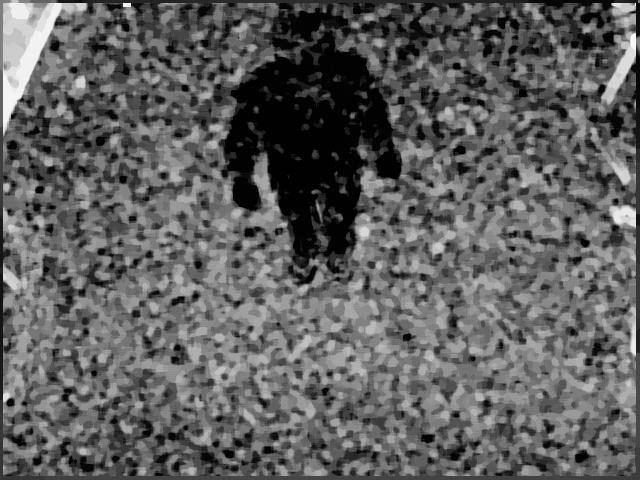
\includegraphics[width=.99\linewidth]{A3/lambda0.5.jpg}
		\caption{$\lambda=0.5$}
	\end{subfigure}
	\begin{subfigure}{.49\textwidth}
		\centering
		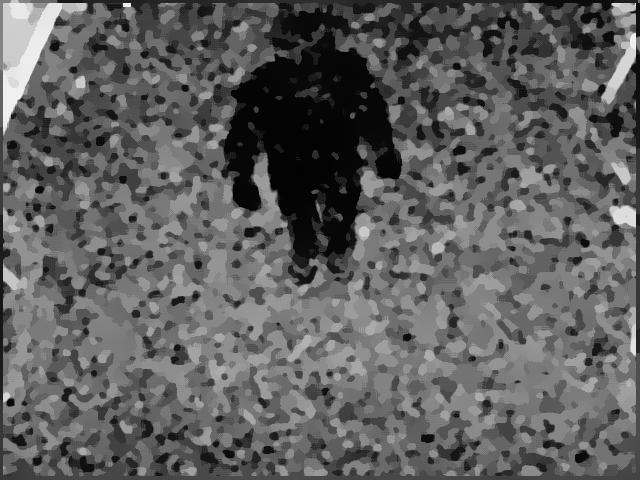
\includegraphics[width=.99\linewidth]{A3/lambda1.jpg}
		\caption{$\lambda=1$}
	\end{subfigure}
	\begin{subfigure}{.49\textwidth}
		\centering
		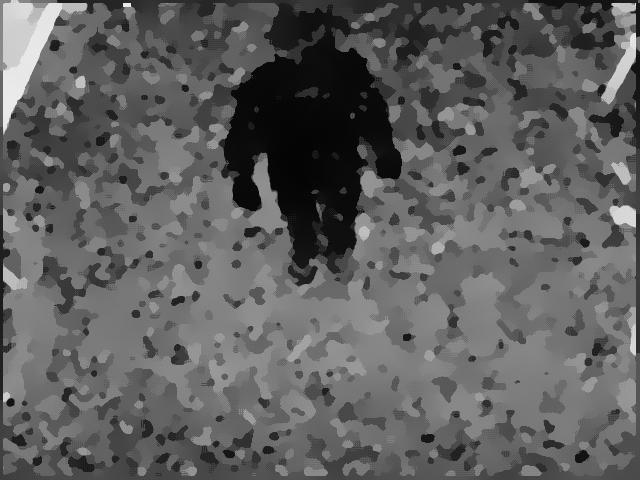
\includegraphics[width=.99\linewidth]{A3/lambda1.5.jpg}
		\caption{$\lambda=1.5$}
	\end{subfigure}
	\begin{subfigure}{.49\textwidth}
		\centering
		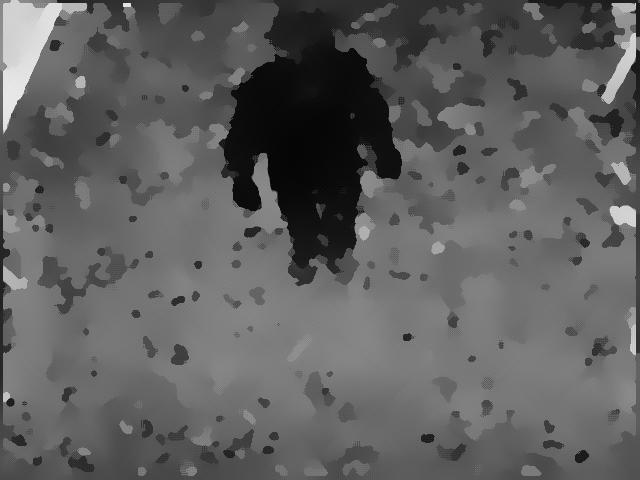
\includegraphics[width=.99\linewidth]{A3/lambda2.jpg}
		\caption{$\lambda=2$}
	\end{subfigure}

	\caption{Isotropes inhomogenes Diffusionsfilter mit $\epsilon_0=1$ und 500 Iterationen}
\end{figure}

\end{document}
